
\chapter{Introduction}

%\Figref{1}
%\fig{awef}{mylabel}

\includegraphics{awef.ps}

\section{Motivation}

It is becoming increasingly important to better manage electricity consumption. Domestic electri- city prices in the UK increased by 35 (in real terms) between 2003 and 2011 [15]. Energy price rises alone are projected to inflate the UK consumer prices index by 1.5 \% in Q4 2011 [17], making energy one of the most dominant upward forces acting on UK consumer prices. This upward price trend is likely to continue as global energy demand, especially from non-OECD countries, contin- ues to grow. In 2000, China used half as much energy as the USA. In 2009, China overtook the USA to become the world�s largest energy user [11]. The International Energy Agency projects that Chinese consumption will increase by 75\% between 2008 and 2035, and that Indian energy consumption will more than double over the same period (although India will still consume less energy in 2035 than either the USA or China) [11].
The UK is especially exposed to energy price rises. The UK makes extensive use of natural gas for heat and power generation. Between 1995 and 2004 the UK was not just self-sufficient for gas but it was also a net exporter of natural gas pumped from the North Sea [20]. Gas production from the North Sea peaked and began its terminal decline in 2000 hence the UK has been a net importer since 2004 [20], requiring us to buy increasing amounts of gas on the volatile global market. Gas production from the North Sea halved between 2000 and 2010 
Text of the Background.

The public are broadly unaware of the finer details of their energy consumption. For example only 17\%

\footnote{\href{http://europa.eu/rapid/pressReleasesAction.do?reference=IP/12/147&format=HTML&aged=0&language=EN&guiLanguage=en}{Europa's Article "Digital Agenda: EU funded project helps citizens compare and reduce their energy consumption via TV, PC and social networks applications"}} 
of people identified the most power hungry appliance in their home (the washing machine) . Pilot projects have demonstrated that mere knowledge of power consumption helps to bring consumption down.
\symbolfootnote{The DEHEMS European Union funded project showed an average reduction of 8\%}

The UK government has made it an explicit goal to increase the understanding of energy usage by users. It has set itself the objective that for every home  and business in Great Britain to have a smart energy meters adapted to their type of usage.

The aim is to begin a national roll out beginning in 2014 and to be completed by 2019. This rollout is to be achieved with the cooperation of the energy industry. It will replace over 53 million gas and electricity meters.

The present project inserts itself into this push by providing a reasoning mechanism to derive information about energy consumption.

Currently however, there are two main aims of deriving information. One is by using a smart meter as aforementioned. The other is by employing an Energy Monitoring Unit. A smart meter is the more accurate of the two options, the monitoring unit only delivering estimated consumption. However a monitoring unit is easy to install and readily available. In this project we will be using a monitoring unit.

The aim of this project is to attempt to profile users based solely on energy readings from an energy monitoring unit.

As the reasoning will be based on a centralised consumption it will remain valid regardless of whether the input is from a smart meter or an energy monitoring unit. A decoupled architecture will ensure that the system can work on both with minor if any modifications.


\section{Smart Meter hardware and Data source}

A large part of this work was spent in data capture and storage.

The constraints.
requirements

The energy monitor chosen is marketed as Current Costs� EnviR. This unit was chosen due to its ease of installation and the clear xml output that it can generate.

You can attach the device to a computer via usb and thus collect discrete xml messages periodically, usually every 6 seconds.


\section{Objectives}


\section{Report outline}



Contributions here.
